% Options for packages loaded elsewhere
\PassOptionsToPackage{unicode}{hyperref}
\PassOptionsToPackage{hyphens}{url}
%
\documentclass[
]{article}
\usepackage{amsmath,amssymb}
\usepackage{iftex}
\ifPDFTeX
  \usepackage[T1]{fontenc}
  \usepackage[utf8]{inputenc}
  \usepackage{textcomp} % provide euro and other symbols
\else % if luatex or xetex
  \usepackage{unicode-math} % this also loads fontspec
  \defaultfontfeatures{Scale=MatchLowercase}
  \defaultfontfeatures[\rmfamily]{Ligatures=TeX,Scale=1}
\fi
\usepackage{lmodern}
\ifPDFTeX\else
  % xetex/luatex font selection
\fi
% Use upquote if available, for straight quotes in verbatim environments
\IfFileExists{upquote.sty}{\usepackage{upquote}}{}
\IfFileExists{microtype.sty}{% use microtype if available
  \usepackage[]{microtype}
  \UseMicrotypeSet[protrusion]{basicmath} % disable protrusion for tt fonts
}{}
\makeatletter
\@ifundefined{KOMAClassName}{% if non-KOMA class
  \IfFileExists{parskip.sty}{%
    \usepackage{parskip}
  }{% else
    \setlength{\parindent}{0pt}
    \setlength{\parskip}{6pt plus 2pt minus 1pt}}
}{% if KOMA class
  \KOMAoptions{parskip=half}}
\makeatother
\usepackage{xcolor}
\usepackage[margin=1in]{geometry}
\usepackage{color}
\usepackage{fancyvrb}
\newcommand{\VerbBar}{|}
\newcommand{\VERB}{\Verb[commandchars=\\\{\}]}
\DefineVerbatimEnvironment{Highlighting}{Verbatim}{commandchars=\\\{\}}
% Add ',fontsize=\small' for more characters per line
\usepackage{framed}
\definecolor{shadecolor}{RGB}{248,248,248}
\newenvironment{Shaded}{\begin{snugshade}}{\end{snugshade}}
\newcommand{\AlertTok}[1]{\textcolor[rgb]{0.94,0.16,0.16}{#1}}
\newcommand{\AnnotationTok}[1]{\textcolor[rgb]{0.56,0.35,0.01}{\textbf{\textit{#1}}}}
\newcommand{\AttributeTok}[1]{\textcolor[rgb]{0.13,0.29,0.53}{#1}}
\newcommand{\BaseNTok}[1]{\textcolor[rgb]{0.00,0.00,0.81}{#1}}
\newcommand{\BuiltInTok}[1]{#1}
\newcommand{\CharTok}[1]{\textcolor[rgb]{0.31,0.60,0.02}{#1}}
\newcommand{\CommentTok}[1]{\textcolor[rgb]{0.56,0.35,0.01}{\textit{#1}}}
\newcommand{\CommentVarTok}[1]{\textcolor[rgb]{0.56,0.35,0.01}{\textbf{\textit{#1}}}}
\newcommand{\ConstantTok}[1]{\textcolor[rgb]{0.56,0.35,0.01}{#1}}
\newcommand{\ControlFlowTok}[1]{\textcolor[rgb]{0.13,0.29,0.53}{\textbf{#1}}}
\newcommand{\DataTypeTok}[1]{\textcolor[rgb]{0.13,0.29,0.53}{#1}}
\newcommand{\DecValTok}[1]{\textcolor[rgb]{0.00,0.00,0.81}{#1}}
\newcommand{\DocumentationTok}[1]{\textcolor[rgb]{0.56,0.35,0.01}{\textbf{\textit{#1}}}}
\newcommand{\ErrorTok}[1]{\textcolor[rgb]{0.64,0.00,0.00}{\textbf{#1}}}
\newcommand{\ExtensionTok}[1]{#1}
\newcommand{\FloatTok}[1]{\textcolor[rgb]{0.00,0.00,0.81}{#1}}
\newcommand{\FunctionTok}[1]{\textcolor[rgb]{0.13,0.29,0.53}{\textbf{#1}}}
\newcommand{\ImportTok}[1]{#1}
\newcommand{\InformationTok}[1]{\textcolor[rgb]{0.56,0.35,0.01}{\textbf{\textit{#1}}}}
\newcommand{\KeywordTok}[1]{\textcolor[rgb]{0.13,0.29,0.53}{\textbf{#1}}}
\newcommand{\NormalTok}[1]{#1}
\newcommand{\OperatorTok}[1]{\textcolor[rgb]{0.81,0.36,0.00}{\textbf{#1}}}
\newcommand{\OtherTok}[1]{\textcolor[rgb]{0.56,0.35,0.01}{#1}}
\newcommand{\PreprocessorTok}[1]{\textcolor[rgb]{0.56,0.35,0.01}{\textit{#1}}}
\newcommand{\RegionMarkerTok}[1]{#1}
\newcommand{\SpecialCharTok}[1]{\textcolor[rgb]{0.81,0.36,0.00}{\textbf{#1}}}
\newcommand{\SpecialStringTok}[1]{\textcolor[rgb]{0.31,0.60,0.02}{#1}}
\newcommand{\StringTok}[1]{\textcolor[rgb]{0.31,0.60,0.02}{#1}}
\newcommand{\VariableTok}[1]{\textcolor[rgb]{0.00,0.00,0.00}{#1}}
\newcommand{\VerbatimStringTok}[1]{\textcolor[rgb]{0.31,0.60,0.02}{#1}}
\newcommand{\WarningTok}[1]{\textcolor[rgb]{0.56,0.35,0.01}{\textbf{\textit{#1}}}}
\usepackage{graphicx}
\makeatletter
\newsavebox\pandoc@box
\newcommand*\pandocbounded[1]{% scales image to fit in text height/width
  \sbox\pandoc@box{#1}%
  \Gscale@div\@tempa{\textheight}{\dimexpr\ht\pandoc@box+\dp\pandoc@box\relax}%
  \Gscale@div\@tempb{\linewidth}{\wd\pandoc@box}%
  \ifdim\@tempb\p@<\@tempa\p@\let\@tempa\@tempb\fi% select the smaller of both
  \ifdim\@tempa\p@<\p@\scalebox{\@tempa}{\usebox\pandoc@box}%
  \else\usebox{\pandoc@box}%
  \fi%
}
% Set default figure placement to htbp
\def\fps@figure{htbp}
\makeatother
\setlength{\emergencystretch}{3em} % prevent overfull lines
\providecommand{\tightlist}{%
  \setlength{\itemsep}{0pt}\setlength{\parskip}{0pt}}
\setcounter{secnumdepth}{-\maxdimen} % remove section numbering
\usepackage{bookmark}
\IfFileExists{xurl.sty}{\usepackage{xurl}}{} % add URL line breaks if available
\urlstyle{same}
\hypersetup{
  pdftitle={Flux\_Calc},
  pdfauthor={Zhang Zhenglin},
  hidelinks,
  pdfcreator={LaTeX via pandoc}}

\title{Flux\_Calc}
\author{Zhang Zhenglin}
\date{}

\begin{document}
\maketitle

{
\setcounter{tocdepth}{2}
\tableofcontents
}
\section{Acknowledgement}\label{acknowledgement}

Heartfelt gratitude to Jack Lamb for providing a functional code
architecture that enabled this to be developed.

\section{Brief overview}\label{brief-overview}

In the field, the start time of each chamber enclosure is recorded.
Chambers are placed on for 4 minutes. This code removes the first and
last minute of chamber enclosures to ensure that the change in
concentration is not subject to disturbance. After which, the data
points are annotated to the respective plots and individual slopes
(ΔC/ΔT) are computed. All linear regressions were inspected to have
R2\textgreater0.85 for the slope to be accepted. ΔC/ΔT is then computed
with chamber parameters including area, volume, and temperature to
determine flux for downstream applications and analyses.

\section{Necessary libraries}\label{necessary-libraries}

\begin{Shaded}
\begin{Highlighting}[]
\FunctionTok{library}\NormalTok{(knitr)}
\FunctionTok{library}\NormalTok{(ggplot2)}
\FunctionTok{theme\_set}\NormalTok{(}\FunctionTok{theme\_bw}\NormalTok{())}
\FunctionTok{library}\NormalTok{(emmeans)}
\FunctionTok{library}\NormalTok{(multcomp)}
\FunctionTok{library}\NormalTok{(PLS205)}
\FunctionTok{library}\NormalTok{(lme4)}
\FunctionTok{library}\NormalTok{(lmerTest)}
\FunctionTok{library}\NormalTok{(multcompView)}
\FunctionTok{library}\NormalTok{(car)}
\FunctionTok{library}\NormalTok{(Rmisc) }
\FunctionTok{library}\NormalTok{(dplyr) }\CommentTok{\#https://r4ds.had.co.nz/ (Chapter 3, Chapter 5, look at filter and select)}
\CommentTok{\# https://bookdown.org/ansellbr/WEHI\_tidyR\_course\_book/}
\FunctionTok{library}\NormalTok{(stringr) }
\FunctionTok{library}\NormalTok{(data.table)}
\FunctionTok{library}\NormalTok{(GGally)}
\FunctionTok{library}\NormalTok{(formatR)}
\FunctionTok{library}\NormalTok{(readxl)}
\FunctionTok{library}\NormalTok{(FluxCalR)}
\FunctionTok{library}\NormalTok{(tidyverse)}
\FunctionTok{library}\NormalTok{(fuzzyjoin)}
\FunctionTok{library}\NormalTok{(purrr)}
\FunctionTok{library}\NormalTok{(data.table)}
\FunctionTok{library}\NormalTok{(broom)}
\FunctionTok{library}\NormalTok{(lubridate)}
\FunctionTok{library}\NormalTok{(readxl)}
\FunctionTok{library}\NormalTok{(openxlsx)}
\FunctionTok{library}\NormalTok{(ggrepel)}
\end{Highlighting}
\end{Shaded}

\section{Entering known parameters of the chamber and set
up}\label{entering-known-parameters-of-the-chamber-and-set-up}

\begin{Shaded}
\begin{Highlighting}[]
\CommentTok{\# volume here expressed at cm3, area in cm2 and height in cm}
\NormalTok{LiCor\_internal\_vol }\OtherTok{\textless{}{-}} \DecValTok{20}
\NormalTok{Chamber\_lid\_height }\OtherTok{\textless{}{-}} \FloatTok{7.62}
\NormalTok{Chamber\_area }\OtherTok{\textless{}{-}}\NormalTok{ pi}\SpecialCharTok{*}\FloatTok{14.75}\SpecialCharTok{*}\FloatTok{14.75}
\end{Highlighting}
\end{Shaded}

\section{Field metadata}\label{field-metadata}

\begin{Shaded}
\begin{Highlighting}[]
\NormalTok{field }\OtherTok{\textless{}{-}} \FunctionTok{read\_excel}\NormalTok{(}\StringTok{"../Field\_Data/Field\_Data.xlsx"}\NormalTok{, }\AttributeTok{sheet =} \DecValTok{1}\NormalTok{)}
\FunctionTok{str}\NormalTok{(field)}
\end{Highlighting}
\end{Shaded}

\begin{verbatim}
## tibble [135 x 10] (S3: tbl_df/tbl/data.frame)
##  $ Plot               : chr [1:135] "E10" "D50" "C50" "B10" ...
##  $ Date               : POSIXct[1:135], format: "2025-06-02" "2025-06-02" ...
##  $ Closure_start_time : POSIXct[1:135], format: NA NA ...
##  $ Chamber_Temp_C     : num [1:135] NA NA NA NA NA NA NA NA NA NA ...
##  $ Headspace_1_cm     : num [1:135] NA NA NA NA NA NA NA NA NA NA ...
##  $ Headspace_2_cm     : num [1:135] NA NA NA NA NA NA NA NA NA NA ...
##  $ Headspace_3_cm     : num [1:135] NA NA NA NA NA NA NA NA NA NA ...
##  $ Headspace_4_cm     : num [1:135] NA NA NA NA NA NA NA NA NA NA ...
##  $ Extension_length_ft: num [1:135] NA NA NA NA NA NA NA NA NA NA ...
##  $ Duration_min       : num [1:135] NA NA NA NA NA NA NA NA NA NA ...
\end{verbatim}

\begin{Shaded}
\begin{Highlighting}[]
\CommentTok{\#chamber volume in cm3 is length multiplied by area. }
\CommentTok{\#Length is given by (sum of chamber lid)+(headspace)+(extension lenght) }
\CommentTok{\#Note that headspace can be negative because floodwater may be above the top of the chamber collar}
\CommentTok{\#We also convert volume from cm3 to L in the calculation below }

\NormalTok{field}\SpecialCharTok{$}\NormalTok{Closure\_datetime\_start }\OtherTok{\textless{}{-}} \FunctionTok{as.POSIXct}\NormalTok{(}
  \FunctionTok{paste}\NormalTok{(field}\SpecialCharTok{$}\NormalTok{Date, }\FunctionTok{format}\NormalTok{(}\FunctionTok{as.POSIXct}\NormalTok{(field}\SpecialCharTok{$}\NormalTok{Closure\_start\_time, }\AttributeTok{format =} \StringTok{"\%Y{-}\%m{-}\%d \%H:\%M:\%S"}\NormalTok{), }\StringTok{"\%H:\%M:\%S"}\NormalTok{)),}
  \AttributeTok{format =} \StringTok{"\%Y{-}\%m{-}\%d \%H:\%M:\%S"}
\NormalTok{)}

\CommentTok{\#Create Closure\_datetime\_end by adding Duration\_min (in minutes) to Closure\_datetime}
\CommentTok{\#now we have the time that the chamber is enclosured by the Li{-}Cor Instrument}
\CommentTok{\#Duration\_min * 60 converts minutes to seconds (because POSIXct handles times in seconds).}
\NormalTok{field}\SpecialCharTok{$}\NormalTok{Closure\_datetime\_end }\OtherTok{\textless{}{-}}\NormalTok{ field}\SpecialCharTok{$}\NormalTok{Closure\_datetime\_start }\SpecialCharTok{+}\NormalTok{ field}\SpecialCharTok{$}\NormalTok{Duration\_min }\SpecialCharTok{*} \DecValTok{60}

\NormalTok{field}\SpecialCharTok{$}\NormalTok{mean\_headspace }\OtherTok{\textless{}{-}} \FunctionTok{rowMeans}\NormalTok{(field[, }\FunctionTok{c}\NormalTok{(}\StringTok{"Headspace\_1\_cm"}\NormalTok{, }\StringTok{"Headspace\_2\_cm"}\NormalTok{, }\StringTok{"Headspace\_3\_cm"}\NormalTok{, }\StringTok{"Headspace\_4\_cm"}\NormalTok{)], }\AttributeTok{na.rm =} \ConstantTok{TRUE}\NormalTok{)}
\NormalTok{field}\SpecialCharTok{$}\NormalTok{Length\_cm }\OtherTok{\textless{}{-}}\NormalTok{ field}\SpecialCharTok{$}\NormalTok{mean\_headspace}\SpecialCharTok{+}\NormalTok{Chamber\_lid\_height}\SpecialCharTok{+}\NormalTok{(field}\SpecialCharTok{$}\NormalTok{Extension\_length\_ft}\SpecialCharTok{*}\FloatTok{30.48}\NormalTok{)}
\NormalTok{field}\SpecialCharTok{$}\NormalTok{Volume\_L }\OtherTok{\textless{}{-}}\NormalTok{ (field}\SpecialCharTok{$}\NormalTok{Length\_cm}\SpecialCharTok{*}\NormalTok{Chamber\_area}\SpecialCharTok{+}\NormalTok{LiCor\_internal\_vol)}\SpecialCharTok{*}\FloatTok{0.001}

\CommentTok{\#remove the first minute and last minute}
\NormalTok{field}\SpecialCharTok{$}\NormalTok{trimmed\_start }\OtherTok{\textless{}{-}}\NormalTok{  field}\SpecialCharTok{$}\NormalTok{Closure\_datetime\_start }\SpecialCharTok{+} \DecValTok{60} 
\NormalTok{field}\SpecialCharTok{$}\NormalTok{trimmed\_end }\OtherTok{\textless{}{-}}\NormalTok{ field}\SpecialCharTok{$}\NormalTok{Closure\_datetime\_end }\SpecialCharTok{{-}} \DecValTok{60}

\FunctionTok{str}\NormalTok{(field)}
\end{Highlighting}
\end{Shaded}

\begin{verbatim}
## tibble [135 x 17] (S3: tbl_df/tbl/data.frame)
##  $ Plot                  : chr [1:135] "E10" "D50" "C50" "B10" ...
##  $ Date                  : POSIXct[1:135], format: "2025-06-02" "2025-06-02" ...
##  $ Closure_start_time    : POSIXct[1:135], format: NA NA ...
##  $ Chamber_Temp_C        : num [1:135] NA NA NA NA NA NA NA NA NA NA ...
##  $ Headspace_1_cm        : num [1:135] NA NA NA NA NA NA NA NA NA NA ...
##  $ Headspace_2_cm        : num [1:135] NA NA NA NA NA NA NA NA NA NA ...
##  $ Headspace_3_cm        : num [1:135] NA NA NA NA NA NA NA NA NA NA ...
##  $ Headspace_4_cm        : num [1:135] NA NA NA NA NA NA NA NA NA NA ...
##  $ Extension_length_ft   : num [1:135] NA NA NA NA NA NA NA NA NA NA ...
##  $ Duration_min          : num [1:135] NA NA NA NA NA NA NA NA NA NA ...
##  $ Closure_datetime_start: POSIXct[1:135], format: NA NA ...
##  $ Closure_datetime_end  : POSIXct[1:135], format: NA NA ...
##  $ mean_headspace        : num [1:135] NaN NaN NaN NaN NaN NaN NaN NaN NaN NaN ...
##  $ Length_cm             : num [1:135] NA NA NA NA NA NA NA NA NA NA ...
##  $ Volume_L              : num [1:135] NA NA NA NA NA NA NA NA NA NA ...
##  $ trimmed_start         : POSIXct[1:135], format: NA NA ...
##  $ trimmed_end           : POSIXct[1:135], format: NA NA ...
\end{verbatim}

\section{Li-Cor Data}\label{li-cor-data}

\subsection{Reading all the relevant Li-Cor
files}\label{reading-all-the-relevant-li-cor-files}

\begin{Shaded}
\begin{Highlighting}[]
\CommentTok{\#so far not needed yet so leaving it here}
\end{Highlighting}
\end{Shaded}

\subsection{Cleaning the master Li-Cor
file}\label{cleaning-the-master-li-cor-file}

\begin{Shaded}
\begin{Highlighting}[]
\NormalTok{raw7810 }\OtherTok{\textless{}{-}} \FunctionTok{read\_tsv}\NormalTok{(}\StringTok{"../Raw\_Licor\_Output\_By\_Day/TG10{-}01532{-}2025{-}05{-}31T090000\_Until\_Jul232025.data"}\NormalTok{,}
                    \AttributeTok{skip =} \DecValTok{5}   \CommentTok{\# skips the first 5 rows      }
\NormalTok{                    ) }\SpecialCharTok{\%\textgreater{}\%}
  \FunctionTok{filter}\NormalTok{(}\SpecialCharTok{!}\FunctionTok{row\_number}\NormalTok{() }\SpecialCharTok{\%in\%} \FunctionTok{c}\NormalTok{(}\DecValTok{1}\NormalTok{))  }\CommentTok{\#removes the units row of the dataframe}
\end{Highlighting}
\end{Shaded}

\begin{verbatim}
## Rows: 95186 Columns: 22
## -- Column specification --------------------------------------------------------
## Delimiter: "\t"
## chr (20): DATAH, SECONDS, NANOSECONDS, NDX, DIAG, DATE, TIME, H2O, CO2, CH4,...
## dbl  (1): RESIDUAL
## lgl  (1): REMARK
## 
## i Use `spec()` to retrieve the full column specification for this data.
## i Specify the column types or set `show_col_types = FALSE` to quiet this message.
\end{verbatim}

\begin{Shaded}
\begin{Highlighting}[]
\CommentTok{\# Combine date and time into a single datetime column, concentration of CH4 is changed from ppm to ppb}
\NormalTok{needed\_data }\OtherTok{\textless{}{-}} \FunctionTok{data.frame}\NormalTok{(}
  \AttributeTok{CH4 =} \FunctionTok{as.numeric}\NormalTok{(raw7810}\SpecialCharTok{$}\NormalTok{CH4)}\SpecialCharTok{*}\FloatTok{0.001}\NormalTok{,}
  \AttributeTok{datetime =} \FunctionTok{as.POSIXct}\NormalTok{(}
    \FunctionTok{paste}\NormalTok{(raw7810}\SpecialCharTok{$}\NormalTok{DATE, raw7810}\SpecialCharTok{$}\NormalTok{TIME),  }\CommentTok{\# Combine date and time strings}
    \AttributeTok{format =} \StringTok{"\%Y{-}\%m{-}\%d \%H:\%M:\%S"}        \CommentTok{\# Adjust format to match data}
\NormalTok{  ),}
  \AttributeTok{residuals =} \FunctionTok{as.numeric}\NormalTok{(raw7810}\SpecialCharTok{$}\NormalTok{RESIDUAL)}
\NormalTok{)}

\NormalTok{needed\_data }\OtherTok{\textless{}{-}}\NormalTok{ needed\_data }\SpecialCharTok{\%\textgreater{}\%}
  \FunctionTok{filter}\NormalTok{(residuals }\SpecialCharTok{\textless{}} \FloatTok{0.025}\NormalTok{) }\SpecialCharTok{\%\textgreater{}\%} \CommentTok{\#removes datapoints where residuals are low}
  \FunctionTok{mutate}\NormalTok{(}
    \AttributeTok{date =} \FunctionTok{as.Date}\NormalTok{(datetime),}
    \AttributeTok{time =} \FunctionTok{format}\NormalTok{(datetime, }\StringTok{"\%H:\%M:\%S"}\NormalTok{)}
\NormalTok{  ) }\SpecialCharTok{\%\textgreater{}\%}
  \FunctionTok{select}\NormalTok{(CH4, date, time, datetime) }

\FunctionTok{str}\NormalTok{(needed\_data)}
\end{Highlighting}
\end{Shaded}

\begin{verbatim}
## 'data.frame':    88964 obs. of  4 variables:
##  $ CH4     : num  NaN NaN NaN NaN NaN NaN NaN NaN NaN NaN ...
##  $ date    : Date, format: "2025-06-01" "2025-06-01" ...
##  $ time    : chr  "15:59:44" "15:59:45" "15:59:46" "15:59:47" ...
##  $ datetime: POSIXct, format: "2025-06-01 15:59:44" "2025-06-01 15:59:45" ...
\end{verbatim}

\subsection{Using field metadata to annotate plots to the Li-Cor
data}\label{using-field-metadata-to-annotate-plots-to-the-li-cor-data}

\begin{Shaded}
\begin{Highlighting}[]
\CommentTok{\# Convert both dataframes to data.tables}
\FunctionTok{setDT}\NormalTok{(needed\_data)}
\FunctionTok{setDT}\NormalTok{(field)}

\CommentTok{\# Perform a non{-}equi join (join where datetime is between trimmed\_start and trimmed\_end)}
\NormalTok{licor\_annotated }\OtherTok{\textless{}{-}}\NormalTok{ field[needed\_data, }
\NormalTok{                         on }\OtherTok{=}\NormalTok{ .(trimmed\_start }\SpecialCharTok{\textless{}=}\NormalTok{ datetime, trimmed\_end }\SpecialCharTok{\textgreater{}=}\NormalTok{ datetime), }
\NormalTok{                         .(datetime, CH4,  Plot), }
\NormalTok{                         nomatch }\OtherTok{=} \DecValTok{0}\NormalTok{]}

\NormalTok{licor\_annotated}\SpecialCharTok{$}\NormalTok{CH4 }\OtherTok{\textless{}{-}} \FunctionTok{as.numeric}\NormalTok{(licor\_annotated}\SpecialCharTok{$}\NormalTok{CH4)}
\NormalTok{licor\_annotated}\SpecialCharTok{$}\NormalTok{Plot }\OtherTok{\textless{}{-}} \FunctionTok{as.factor}\NormalTok{(licor\_annotated}\SpecialCharTok{$}\NormalTok{Plot)}

\FunctionTok{str}\NormalTok{(licor\_annotated)}
\end{Highlighting}
\end{Shaded}

\begin{verbatim}
## Classes 'data.table' and 'data.frame':   7200 obs. of  3 variables:
##  $ datetime: POSIXct, format: "2025-06-18 09:33:00" "2025-06-18 09:33:01" ...
##  $ CH4     : num  5.61 5.62 5.64 5.65 5.67 ...
##  $ Plot    : Factor w/ 15 levels "A0","A10","A50",..: 14 14 14 14 14 14 14 14 14 14 ...
##  - attr(*, ".internal.selfref")=<externalptr>
\end{verbatim}

\section{Flux calculation}\label{flux-calculation}

\subsection{Function that calculates change in CH4 concentration over
time
(ppm/s)}\label{function-that-calculates-change-in-ch4-concentration-over-time-ppms}

\begin{Shaded}
\begin{Highlighting}[]
\NormalTok{get\_CH4\_slopes }\OtherTok{\textless{}{-}} \ControlFlowTok{function}\NormalTok{(data) \{}
\NormalTok{  data }\SpecialCharTok{\%\textgreater{}\%}
    \FunctionTok{mutate}\NormalTok{(}
      \AttributeTok{date =} \FunctionTok{as.Date}\NormalTok{(datetime),}
      \AttributeTok{datetime\_num =} \FunctionTok{as.numeric}\NormalTok{(datetime) }\SpecialCharTok{{-}} \FunctionTok{min}\NormalTok{(}\FunctionTok{as.numeric}\NormalTok{(datetime), }\AttributeTok{na.rm =} \ConstantTok{TRUE}\NormalTok{)}
\NormalTok{    ) }\SpecialCharTok{\%\textgreater{}\%}
    \FunctionTok{group\_by}\NormalTok{(Plot, date) }\SpecialCharTok{\%\textgreater{}\%}
    \FunctionTok{group\_split}\NormalTok{() }\SpecialCharTok{\%\textgreater{}\%}
    \FunctionTok{map\_dfr}\NormalTok{(}\ControlFlowTok{function}\NormalTok{(df) \{}
      \ControlFlowTok{if}\NormalTok{ (}\FunctionTok{nrow}\NormalTok{(df) }\SpecialCharTok{\textless{}} \DecValTok{2} \SpecialCharTok{||} \FunctionTok{all}\NormalTok{(}\FunctionTok{is.na}\NormalTok{(df}\SpecialCharTok{$}\NormalTok{CH4))) \{}
        \FunctionTok{return}\NormalTok{(}\FunctionTok{tibble}\NormalTok{(}
          \AttributeTok{Plot =}\NormalTok{ df}\SpecialCharTok{$}\NormalTok{Plot[}\DecValTok{1}\NormalTok{],}
          \AttributeTok{date =}\NormalTok{ df}\SpecialCharTok{$}\NormalTok{date[}\DecValTok{1}\NormalTok{],}
          \CommentTok{\#n = nrow(df),}
          \CommentTok{\#n\_ch4 = sum(!is.na(df$CH4)),}
          \AttributeTok{time\_span =} \FunctionTok{as.numeric}\NormalTok{(}\FunctionTok{difftime}\NormalTok{(}\FunctionTok{max}\NormalTok{(df}\SpecialCharTok{$}\NormalTok{datetime), }\FunctionTok{min}\NormalTok{(df}\SpecialCharTok{$}\NormalTok{datetime), }\AttributeTok{units =} \StringTok{"secs"}\NormalTok{)),}
          \CommentTok{\#ch4\_var = var(df$CH4, na.rm = TRUE),}
          \AttributeTok{slope =} \ConstantTok{NA\_real\_}\NormalTok{,}
          \AttributeTok{r\_squared =} \ConstantTok{NA\_real\_}
\NormalTok{        ))}
\NormalTok{      \}}
      
\NormalTok{      model }\OtherTok{\textless{}{-}} \FunctionTok{tryCatch}\NormalTok{(}\FunctionTok{lm}\NormalTok{(CH4 }\SpecialCharTok{\textasciitilde{}}\NormalTok{ datetime\_num, }\AttributeTok{data =}\NormalTok{ df), }\AttributeTok{error =} \ControlFlowTok{function}\NormalTok{(e) }\ConstantTok{NULL}\NormalTok{)}
      
      \ControlFlowTok{if}\NormalTok{ (}\FunctionTok{is.null}\NormalTok{(model)) \{}
\NormalTok{        slope }\OtherTok{\textless{}{-}} \ConstantTok{NA\_real\_}
\NormalTok{        r2 }\OtherTok{\textless{}{-}} \ConstantTok{NA\_real\_}
\NormalTok{      \} }\ControlFlowTok{else}\NormalTok{ \{}
\NormalTok{        slope }\OtherTok{\textless{}{-}} \FunctionTok{coef}\NormalTok{(model)[}\StringTok{"datetime\_num"}\NormalTok{]}
\NormalTok{        r2 }\OtherTok{\textless{}{-}} \FunctionTok{summary}\NormalTok{(model)}\SpecialCharTok{$}\NormalTok{r.squared}
\NormalTok{      \}}
      
      \FunctionTok{tibble}\NormalTok{(}
        \AttributeTok{Plot =}\NormalTok{ df}\SpecialCharTok{$}\NormalTok{Plot[}\DecValTok{1}\NormalTok{],}
        \AttributeTok{date =}\NormalTok{ df}\SpecialCharTok{$}\NormalTok{date[}\DecValTok{1}\NormalTok{],}
        \CommentTok{\#n = nrow(df),}
        \CommentTok{\#n\_ch4 = sum(!is.na(df$CH4)),}
        \AttributeTok{time\_span =} \FunctionTok{as.numeric}\NormalTok{(}\FunctionTok{difftime}\NormalTok{(}\FunctionTok{max}\NormalTok{(df}\SpecialCharTok{$}\NormalTok{datetime), }\FunctionTok{min}\NormalTok{(df}\SpecialCharTok{$}\NormalTok{datetime), }\AttributeTok{units =} \StringTok{"secs"}\NormalTok{)),}
        \CommentTok{\#ch4\_var = var(df$CH4, na.rm = TRUE),}
        \AttributeTok{slope =}\NormalTok{ slope,}
        \AttributeTok{r\_squared =}\NormalTok{ r2}
\NormalTok{      )}
\NormalTok{    \})}
\NormalTok{\}}
\end{Highlighting}
\end{Shaded}

\subsection{Get CH4 slopes (ppm/s)}\label{get-ch4-slopes-ppms}

\begin{Shaded}
\begin{Highlighting}[]
\NormalTok{all\_fluxes}\OtherTok{\textless{}{-}} \FunctionTok{get\_CH4\_slopes}\NormalTok{(licor\_annotated)}
\end{Highlighting}
\end{Shaded}

\section{Calculate flux}\label{calculate-flux}

\subsection{Going from change in concentration to
flux}\label{going-from-change-in-concentration-to-flux}

\begin{figure}
\centering
\pandocbounded{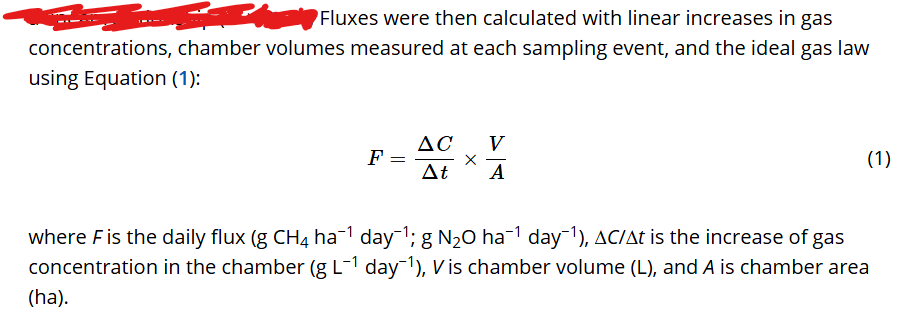
\includegraphics[keepaspectratio]{C:/Users/zhang/Documents/GitHub/ERW/Scripts/Flux_Equation.png}}
\caption{Equation for calcualting flux}
\end{figure}

Zhang, Z., Fenster, T. L. D., \& Linquist, B. A. (2025). Greenhouse gas
emissions altered by the introduction of a year-long fallow to
continuous rice systems. Journal of Environmental Quality, 1--15.
\url{https://doi.org/10.1002/jeq2.70055}

\begin{Shaded}
\begin{Highlighting}[]
\CommentTok{\#get temperature,volume, and chamber area from field metadata}
\NormalTok{all\_fluxes}\SpecialCharTok{$}\NormalTok{Date }\OtherTok{\textless{}{-}}\NormalTok{ all\_fluxes}\SpecialCharTok{$}\NormalTok{date}

\NormalTok{all\_fluxes }\OtherTok{\textless{}{-}}\NormalTok{ all\_fluxes }\SpecialCharTok{\%\textgreater{}\%}
  \FunctionTok{left\_join}\NormalTok{(field }\SpecialCharTok{\%\textgreater{}\%} \FunctionTok{select}\NormalTok{(Date, Plot, Volume\_L, Chamber\_Temp\_C), }
            \AttributeTok{by =} \FunctionTok{c}\NormalTok{(}\StringTok{"Date"}\NormalTok{, }\StringTok{"Plot"}\NormalTok{)) }\SpecialCharTok{\%\textgreater{}\%}
  \FunctionTok{mutate}\NormalTok{(}\AttributeTok{Area=}\NormalTok{Chamber\_area}\SpecialCharTok{/}\DecValTok{100000000}\NormalTok{) }\CommentTok{\#changing from cm2 to ha}


\CommentTok{\# this is to convert change in concentration over time from ppm/s (all\_fluxes$slope) to mg L{-}1 s{-}1 using ideal gas law}
\NormalTok{all\_fluxes}\SpecialCharTok{$}\NormalTok{slope\_mg\_L\_s }\OtherTok{\textless{}{-}}\NormalTok{ (((all\_fluxes}\SpecialCharTok{$}\NormalTok{slope)}\SpecialCharTok{/}\NormalTok{((((}\DecValTok{760}\SpecialCharTok{*}\FloatTok{22.4}\NormalTok{)}\SpecialCharTok{*}\NormalTok{(}\DecValTok{273}\SpecialCharTok{+}\NormalTok{all\_fluxes}\SpecialCharTok{$}\NormalTok{Chamber\_Temp\_C))}\SpecialCharTok{/}\NormalTok{(}\DecValTok{760}\SpecialCharTok{*}\DecValTok{273}\NormalTok{))))}\SpecialCharTok{*}\NormalTok{(}\FloatTok{0.016043}\NormalTok{))}

\CommentTok{\# get flux with chamber volume and area. Scale from mg/s to mg/d}
\NormalTok{all\_fluxes}\SpecialCharTok{$}\NormalTok{CH4\_flux\_g\_ha\_day }\OtherTok{\textless{}{-}}\NormalTok{ ((all\_fluxes}\SpecialCharTok{$}\NormalTok{slope\_mg\_L\_s)}\SpecialCharTok{/}\NormalTok{(all\_fluxes}\SpecialCharTok{$}\NormalTok{Area))}\SpecialCharTok{*}\NormalTok{(all\_fluxes}\SpecialCharTok{$}\NormalTok{Volume\_L)}\SpecialCharTok{*}\DecValTok{86400}\SpecialCharTok{*}\FloatTok{0.001}

\NormalTok{all\_fluxes}\SpecialCharTok{$}\NormalTok{CH4\_flux\_g\_ha\_day\_all\_in\_one }\OtherTok{\textless{}{-}}\NormalTok{ ((((all\_fluxes}\SpecialCharTok{$}\NormalTok{slope)}\SpecialCharTok{/}\NormalTok{((((}\DecValTok{760}\SpecialCharTok{*}\FloatTok{22.4}\NormalTok{)}\SpecialCharTok{*}\NormalTok{(}\DecValTok{273}\SpecialCharTok{+}\NormalTok{all\_fluxes}\SpecialCharTok{$}\NormalTok{Chamber\_Temp\_C))}\SpecialCharTok{/}\NormalTok{(}\DecValTok{760}\SpecialCharTok{*}\DecValTok{273}\NormalTok{))))}\SpecialCharTok{*}\NormalTok{(}\FloatTok{0.016043}\NormalTok{))}\SpecialCharTok{/}\NormalTok{(all\_fluxes}\SpecialCharTok{$}\NormalTok{Area))}\SpecialCharTok{*}\NormalTok{(all\_fluxes}\SpecialCharTok{$}\NormalTok{Volume\_L)}\SpecialCharTok{*}\DecValTok{86400}\SpecialCharTok{*}\FloatTok{0.001}
\end{Highlighting}
\end{Shaded}

\section{Compiling data and quality
check}\label{compiling-data-and-quality-check}

\subsection{Create final dataframe with plot, flux, and date for
downstream
applications}\label{create-final-dataframe-with-plot-flux-and-date-for-downstream-applications}

\begin{Shaded}
\begin{Highlighting}[]
\NormalTok{final\_flux }\OtherTok{\textless{}{-}}\NormalTok{ all\_fluxes }\SpecialCharTok{\%\textgreater{}\%} 
  \FunctionTok{select}\NormalTok{(Plot, Date, CH4\_flux\_g\_ha\_day) }\SpecialCharTok{\%\textgreater{}\%}
  \FunctionTok{mutate}\NormalTok{(}\AttributeTok{Treatment =} \FunctionTok{factor}\NormalTok{(}\FunctionTok{str\_sub}\NormalTok{(Plot, }\DecValTok{2}\NormalTok{)))}
  
\FunctionTok{str}\NormalTok{(final\_flux)}
\end{Highlighting}
\end{Shaded}

\begin{verbatim}
## tibble [60 x 4] (S3: tbl_df/tbl/data.frame)
##  $ Plot             : chr [1:60] "A0" "A0" "A0" "A0" ...
##  $ Date             : POSIXct[1:60], format: "2025-06-18" "2025-06-27" ...
##  $ CH4_flux_g_ha_day: Named num [1:60] 2947 714 697 1175 5848 ...
##   ..- attr(*, "names")= chr [1:60] "datetime_num" "datetime_num" "datetime_num" "datetime_num" ...
##  $ Treatment        : Factor w/ 3 levels "0","10","50": 1 1 1 1 2 2 2 2 3 3 ...
\end{verbatim}

\begin{Shaded}
\begin{Highlighting}[]
\FunctionTok{write.xlsx}\NormalTok{(all\_fluxes, }\AttributeTok{file=} \StringTok{"../Computed\_Flux/all\_fluxes.xlsx"}\NormalTok{, }\AttributeTok{sheetName =} \StringTok{"1"}\NormalTok{, }\AttributeTok{rowNames =} \ConstantTok{FALSE}\NormalTok{)}
\end{Highlighting}
\end{Shaded}

\subsection{Create PDF with all the plots to visually inspect change in
concentration over time is
linear}\label{create-pdf-with-all-the-plots-to-visually-inspect-change-in-concentration-over-time-is-linear}

\begin{Shaded}
\begin{Highlighting}[]
\CommentTok{\# Create a Date column}
\NormalTok{licor\_annotated }\OtherTok{\textless{}{-}}\NormalTok{ licor\_annotated }\SpecialCharTok{\%\textgreater{}\%}
  \FunctionTok{mutate}\NormalTok{(}\AttributeTok{Date =} \FunctionTok{as.Date}\NormalTok{(datetime))}

\CommentTok{\# Open PDF device}
\FunctionTok{pdf}\NormalTok{(}\StringTok{"../Figures/CH4\_time\_series\_by\_date.pdf"}\NormalTok{, }\AttributeTok{width =} \DecValTok{10}\NormalTok{, }\AttributeTok{height =} \DecValTok{6}\NormalTok{)}

\CommentTok{\# Loop over every 2 dates (i.e., 2 plots per page)}
\NormalTok{dates }\OtherTok{\textless{}{-}} \FunctionTok{unique}\NormalTok{(licor\_annotated}\SpecialCharTok{$}\NormalTok{Date)}

\ControlFlowTok{for}\NormalTok{ (i }\ControlFlowTok{in} \FunctionTok{seq}\NormalTok{(}\DecValTok{1}\NormalTok{, }\FunctionTok{length}\NormalTok{(dates), }\AttributeTok{by =} \DecValTok{2}\NormalTok{)) \{}
  
  \CommentTok{\# Get current chunk of 1 or 2 dates}
\NormalTok{  current\_dates }\OtherTok{\textless{}{-}}\NormalTok{ dates[i}\SpecialCharTok{:}\FunctionTok{min}\NormalTok{(i}\SpecialCharTok{+}\DecValTok{1}\NormalTok{, }\FunctionTok{length}\NormalTok{(dates))]}
\NormalTok{  plot\_data }\OtherTok{\textless{}{-}}\NormalTok{ licor\_annotated }\SpecialCharTok{\%\textgreater{}\%} \FunctionTok{filter}\NormalTok{(Date }\SpecialCharTok{\%in\%}\NormalTok{ current\_dates)}

\NormalTok{  p }\OtherTok{\textless{}{-}} \FunctionTok{ggplot}\NormalTok{(plot\_data, }\FunctionTok{aes}\NormalTok{(}\AttributeTok{x =}\NormalTok{ datetime, }\AttributeTok{y =}\NormalTok{ CH4, }\AttributeTok{color =}\NormalTok{ Plot, }\AttributeTok{group =}\NormalTok{ Plot)) }\SpecialCharTok{+}
    \FunctionTok{geom\_point}\NormalTok{(}\AttributeTok{size=}\FloatTok{0.5}\NormalTok{) }\SpecialCharTok{+}
    \FunctionTok{facet\_wrap}\NormalTok{(}\SpecialCharTok{\textasciitilde{}}\NormalTok{ Date, }\AttributeTok{ncol =} \DecValTok{1}\NormalTok{, }\AttributeTok{scales =} \StringTok{"free\_x"}\NormalTok{) }\SpecialCharTok{+}
    \CommentTok{\#ylim(0, 20) +   }
    \FunctionTok{labs}\NormalTok{(}\AttributeTok{title =} \StringTok{"CH₄ concentration over time"}\NormalTok{,}
         \AttributeTok{x =} \StringTok{"Time"}\NormalTok{,}
         \AttributeTok{y =} \StringTok{"CH₄ (ppm)"}\NormalTok{) }\SpecialCharTok{+}
    \FunctionTok{theme\_minimal}\NormalTok{(}\AttributeTok{base\_size =} \DecValTok{14}\NormalTok{) }\SpecialCharTok{+}
    \FunctionTok{theme}\NormalTok{(}
      \AttributeTok{plot.title =} \FunctionTok{element\_text}\NormalTok{(}\AttributeTok{hjust =} \FloatTok{0.5}\NormalTok{, }\AttributeTok{face =} \StringTok{"bold"}\NormalTok{),}
      \AttributeTok{legend.position =} \StringTok{"bottom"}
\NormalTok{    )}
  
  \FunctionTok{print}\NormalTok{(p)}
\NormalTok{\}}

\FunctionTok{dev.off}\NormalTok{()}
\end{Highlighting}
\end{Shaded}

\begin{verbatim}
## pdf 
##   2
\end{verbatim}

\end{document}
